%%%%%%%%%%%%%%%%%%%%%%%%%%%%%%%%%%%%%%%%%
% The Legrand Orange Book
% LaTeX Template
% Version 2.1.1 (14/2/16)
%
% This template has been downloaded from:
% http://www.LaTeXTemplates.com
%
% Original author:
% Mathias Legrand (legrand.mathias@gmail.com) with modifications by:
% Vel (vel@latextemplates.com)
%
% License:
% CC BY-NC-SA 3.0 (http://creativecommons.org/licenses/by-nc-sa/3.0/)
%
% Compiling this template:
% This template uses biber for its bibliography and makeindex for its index.
% When you first open the template, compile it from the command line with the 
% commands below to make sure your LaTeX distribution is configured correctly:
%
% 1) pdflatex main
% 2) makeindex main.idx -s StyleInd.ist
% 3) biber main
% 4) pdflatex main x 2
%
% After this, when you wish to update the bibliography/index use the appropriate
% command above and make sure to compile with pdflatex several times 
% afterwards to propagate your changes to the document.
%
% This template also uses a number of packages which may need to be
% updated to the newest versions for the template to compile. It is strongly
% recommended you update your LaTeX distribution if you have any
% compilation errors.
%
% Important note:
% Chapter heading images should have a 2:1 width:height ratio,
% e.g. 920px width and 460px height.
%
%%%%%%%%%%%%%%%%%%%%%%%%%%%%%%%%%%%%%%%%%

%----------------------------------------------------------------------------------------
%	PACKAGES AND OTHER DOCUMENT CONFIGURATIONS
%----------------------------------------------------------------------------------------

\documentclass[11pt,fleqn]{book} % Default font size and left-justified equations

%----------------------------------------------------------------------------------------

%%%%%%%%%%%%%%%%%%%%%%%%%%%%%%%%%%%%%%%%%
% The Legrand Orange Book
% Structural Definitions File
% Version 2.0 (9/2/15)
%
% Original author:
% Mathias Legrand (legrand.mathias@gmail.com) with modifications by:
% Vel (vel@latextemplates.com)
% 
% This file has been downloaded from:
% http://www.LaTeXTemplates.com
%
% License:
% CC BY-NC-SA 3.0 (http://creativecommons.org/licenses/by-nc-sa/3.0/)
%
%%%%%%%%%%%%%%%%%%%%%%%%%%%%%%%%%%%%%%%%%

%----------------------------------------------------------------------------------------
%	VARIOUS REQUIRED PACKAGES AND CONFIGURATIONS
%----------------------------------------------------------------------------------------

\usepackage[top=3cm,bottom=3cm,left=3cm,right=3cm,headsep=10pt,a4paper]{geometry} % Page margins

\usepackage{graphicx} % Required for including pictures
\graphicspath{{Pictures/}} % Specifies the directory where pictures are stored

\usepackage{tikz} % Required for drawing

\usepackage{pgfplots}
\pgfplotsset{width=10cm,compat=1.9}

\usepackage{circuitikz}

\usepackage{lipsum} % Inserts dummy text

\usepackage{tikz} % Required for drawing custom shapes

\usepackage[brazilian]{babel} % Pt-br language/hyphenation

\usepackage{enumitem} % Customize lists
\setlist{nolistsep} % Reduce spacing between bullet points and numbered lists

\usepackage{booktabs} % Required for nicer horizontal rules in tables

\usepackage{xcolor} % Required for specifying colors by name
\definecolor{ocre}{RGB}{0,104,179} % Define the orange color used for highlighting throughout the book

%----------------------------------------------------------------------------------------
%	FONTS
%----------------------------------------------------------------------------------------

\usepackage{avant} % Use the Avantgarde font for headings
%\usepackage{times} % Use the Times font for headings
\usepackage{mathptmx} % Use the Adobe Times Roman as the default text font together with math symbols from the Sym­bol, Chancery and Com­puter Modern fonts

\usepackage{microtype} % Slightly tweak font spacing for aesthetics
\usepackage[utf8]{inputenc} % Required for including letters with accents
\usepackage[T1]{fontenc} % Use 8-bit encoding that has 256 glyphs

%----------------------------------------------------------------------------------------
%	BIBLIOGRAPHY AND INDEX
%----------------------------------------------------------------------------------------

\usepackage[style=alphabetic,citestyle=numeric,sorting=nyt,sortcites=true,autopunct=true,babel=hyphen,hyperref=true,abbreviate=false,backref=true,backend=biber]{biblatex}
\addbibresource{bibliography.bib} % BibTeX bibliography file
\defbibheading{bibempty}{}

\usepackage{calc} % For simpler calculation - used for spacing the index letter headings correctly
\usepackage{makeidx} % Required to make an index
\makeindex % Tells LaTeX to create the files required for indexing

%----------------------------------------------------------------------------------------
%	MAIN TABLE OF CONTENTS
%----------------------------------------------------------------------------------------

\usepackage{titletoc} % Required for manipulating the table of contents

\contentsmargin{0cm} % Removes the default margin

% Part text styling
\titlecontents{part}[0cm]
{\addvspace{20pt}\centering\large\bfseries}
{}
{}
{}

% Chapter text styling
\titlecontents{chapter}[1.25cm] % Indentation
{\addvspace{12pt}\large\sffamily\bfseries} % Spacing and font options for chapters
{\color{ocre!60}\contentslabel[\Large\thecontentslabel]{1.25cm}\color{ocre}} % Chapter number
{\color{ocre}}  
{\color{ocre!60}\normalsize\;\titlerule*[.5pc]{.}\;\thecontentspage} % Page number

% Section text styling
\titlecontents{section}[1.25cm] % Indentation
{\addvspace{3pt}\sffamily\bfseries} % Spacing and font options for sections
{\contentslabel[\thecontentslabel]{1.25cm}} % Section number
{}
{\hfill\color{black}\thecontentspage} % Page number
[]

% Subsection text styling
\titlecontents{subsection}[1.25cm] % Indentation
{\addvspace{1pt}\sffamily\small} % Spacing and font options for subsections
{\contentslabel[\thecontentslabel]{1.25cm}} % Subsection number
{}
{\ \titlerule*[.5pc]{.}\;\thecontentspage} % Page number
[]

% List of figures
\titlecontents{figure}[0em]
{\addvspace{-5pt}\sffamily}
{\thecontentslabel\hspace*{1em}}
{}
{\ \titlerule*[.5pc]{.}\;\thecontentspage}
[]

% List of tables
\titlecontents{table}[0em]
{\addvspace{-5pt}\sffamily}
{\thecontentslabel\hspace*{1em}}
{}
{\ \titlerule*[.5pc]{.}\;\thecontentspage}
[]

%----------------------------------------------------------------------------------------
%	MINI TABLE OF CONTENTS IN PART HEADS
%----------------------------------------------------------------------------------------

% Chapter text styling
\titlecontents{lchapter}[0em] % Indenting
{\addvspace{15pt}\large\sffamily\bfseries} % Spacing and font options for chapters
{\color{ocre}\contentslabel[\Large\thecontentslabel]{1.25cm}\color{ocre}} % Chapter number
{}  
{\color{ocre}\normalsize\sffamily\bfseries\;\titlerule*[.5pc]{.}\;\thecontentspage} % Page number

% Section text styling
\titlecontents{lsection}[0em] % Indenting
{\sffamily\small} % Spacing and font options for sections
{\contentslabel[\thecontentslabel]{1.25cm}} % Section number
{}
{}

% Subsection text styling
\titlecontents{lsubsection}[.5em] % Indentation
{\normalfont\footnotesize\sffamily} % Font settings
{}
{}
{}

%----------------------------------------------------------------------------------------
%	PAGE HEADERS
%----------------------------------------------------------------------------------------

\usepackage{fancyhdr} % Required for header and footer configuration

\pagestyle{fancy}
\renewcommand{\chaptermark}[1]{\markboth{\sffamily\normalsize\bfseries\chaptername\ \thechapter.\ #1}{}} % Chapter text font settings
\renewcommand{\sectionmark}[1]{\markright{\sffamily\normalsize\thesection\hspace{5pt}#1}{}} % Section text font settings
\fancyhf{} \fancyhead[LE,RO]{\sffamily\normalsize\thepage} % Font setting for the page number in the header
\fancyhead[LO]{\rightmark} % Print the nearest section name on the left side of odd pages
\fancyhead[RE]{\leftmark} % Print the current chapter name on the right side of even pages
\renewcommand{\headrulewidth}{0.5pt} % Width of the rule under the header
\addtolength{\headheight}{2.5pt} % Increase the spacing around the header slightly
\renewcommand{\footrulewidth}{0pt} % Removes the rule in the footer
\fancypagestyle{plain}{\fancyhead{}\renewcommand{\headrulewidth}{0pt}} % Style for when a plain pagestyle is specified

% Removes the header from odd empty pages at the end of chapters
\makeatletter
\renewcommand{\cleardoublepage}{
\clearpage\ifodd\c@page\else
\hbox{}
\vspace*{\fill}
\thispagestyle{empty}
\newpage
\fi}

%----------------------------------------------------------------------------------------
%	THEOREM STYLES
%----------------------------------------------------------------------------------------

\usepackage{amsmath,amsfonts,amssymb,amsthm} % For math equations, theorems, symbols, etc

\newcommand{\intoo}[2]{\mathopen{]}#1\,;#2\mathclose{[}}
\newcommand{\ud}{\mathop{\mathrm{{}d}}\mathopen{}}
\newcommand{\intff}[2]{\mathopen{[}#1\,;#2\mathclose{]}}
\newtheorem{notation}{Notation}[chapter]

% Boxed/framed environments
\newtheoremstyle{ocrenumbox}% % Theorem style name
{0pt}% Space above
{0pt}% Space below
{\normalfont}% % Body font
{}% Indent amount
{\small\bf\sffamily\color{ocre}}% % Theorem head font
{\;}% Punctuation after theorem head
{0.25em}% Space after theorem head
{\small\sffamily\color{ocre}\thmname{#1}\nobreakspace\thmnumber{\@ifnotempty{#1}{}\@upn{#2}}% Theorem text (e.g. Theorem 2.1)
\thmnote{\nobreakspace\the\thm@notefont\sffamily\bfseries\color{black}---\nobreakspace#3.}} % Optional theorem note
\renewcommand{\qedsymbol}{$\blacksquare$}% Optional qed square

\newtheoremstyle{blacknumex}% Theorem style name
{5pt}% Space above
{5pt}% Space below
{\normalfont}% Body font
{} % Indent amount
{\small\bf\sffamily}% Theorem head font
{\;}% Punctuation after theorem head
{0.25em}% Space after theorem head
{\small\sffamily{\tiny\ensuremath{\blacksquare}}\nobreakspace\thmname{#1}\nobreakspace\thmnumber{\@ifnotempty{#1}{}\@upn{#2}}% Theorem text (e.g. Theorem 2.1)
\thmnote{\nobreakspace\the\thm@notefont\sffamily\bfseries---\nobreakspace#3.}}% Optional theorem note

\newtheoremstyle{blacknumbox} % Theorem style name
{0pt}% Space above
{0pt}% Space below
{\normalfont}% Body font
{}% Indent amount
{\small\bf\sffamily}% Theorem head font
{\;}% Punctuation after theorem head
{0.25em}% Space after theorem head
{\small\sffamily\thmname{#1}\nobreakspace\thmnumber{\@ifnotempty{#1}{}\@upn{#2}}% Theorem text (e.g. Theorem 2.1)
\thmnote{\nobreakspace\the\thm@notefont\sffamily\bfseries---\nobreakspace#3.}}% Optional theorem note

% Non-boxed/non-framed environments
\newtheoremstyle{ocrenum}% % Theorem style name
{5pt}% Space above
{5pt}% Space below
{\normalfont}% % Body font
{}% Indent amount
{\small\bf\sffamily\color{ocre}}% % Theorem head font
{\;}% Punctuation after theorem head
{0.25em}% Space after theorem head
{\small\sffamily\color{ocre}\thmname{#1}\nobreakspace\thmnumber{\@ifnotempty{#1}{}\@upn{#2}}% Theorem text (e.g. Theorem 2.1)
\thmnote{\nobreakspace\the\thm@notefont\sffamily\bfseries\color{black}---\nobreakspace#3.}} % Optional theorem note
\renewcommand{\qedsymbol}{$\blacksquare$}% Optional qed square
\makeatother

% Defines the theorem text style for each type of theorem to one of the three styles above
\newcounter{dummy} 
\numberwithin{dummy}{section}
\theoremstyle{ocrenumbox}
\newtheorem{theoremeT}[dummy]{Theorem}
\newtheorem{problem}{Problem}[chapter]
\newtheorem{exerciseT}{Exercise}[chapter]
\theoremstyle{blacknumex}
\newtheorem{exampleT}{Example}[chapter]
\theoremstyle{blacknumbox}
\newtheorem{vocabulary}{Vocabulary}[chapter]
\newtheorem{definitionT}{Definition}[section]
\newtheorem{corollaryT}[dummy]{Corollary}
\theoremstyle{ocrenum}
\newtheorem{proposition}[dummy]{Proposition}

%----------------------------------------------------------------------------------------
%	DEFINITION OF COLORED BOXES
%----------------------------------------------------------------------------------------

\RequirePackage[framemethod=default]{mdframed} % Required for creating the theorem, definition, exercise and corollary boxes

% Theorem box
\newmdenv[skipabove=7pt,
skipbelow=7pt,
backgroundcolor=black!5,
linecolor=ocre,
innerleftmargin=5pt,
innerrightmargin=5pt,
innertopmargin=5pt,
leftmargin=0cm,
rightmargin=0cm,
innerbottommargin=5pt]{tBox}

% Exercise box	  
\newmdenv[skipabove=7pt,
skipbelow=7pt,
rightline=false,
leftline=true,
topline=false,
bottomline=false,
backgroundcolor=ocre!10,
linecolor=ocre,
innerleftmargin=5pt,
innerrightmargin=5pt,
innertopmargin=5pt,
innerbottommargin=5pt,
leftmargin=0cm,
rightmargin=0cm,
linewidth=4pt]{eBox}	

% Definition box
\newmdenv[skipabove=7pt,
skipbelow=7pt,
rightline=false,
leftline=true,
topline=false,
bottomline=false,
linecolor=ocre,
innerleftmargin=5pt,
innerrightmargin=5pt,
innertopmargin=0pt,
leftmargin=0cm,
rightmargin=0cm,
linewidth=4pt,
innerbottommargin=0pt]{dBox}	

% Corollary box
\newmdenv[skipabove=7pt,
skipbelow=7pt,
rightline=false,
leftline=true,
topline=false,
bottomline=false,
linecolor=gray,
backgroundcolor=black!5,
innerleftmargin=5pt,
innerrightmargin=5pt,
innertopmargin=5pt,
leftmargin=0cm,
rightmargin=0cm,
linewidth=4pt,
innerbottommargin=5pt]{cBox}

% Creates an environment for each type of theorem and assigns it a theorem text style from the "Theorem Styles" section above and a colored box from above
\newenvironment{theorem}{\begin{tBox}\begin{theoremeT}}{\end{theoremeT}\end{tBox}}
\newenvironment{exercise}{\begin{eBox}\begin{exerciseT}}{\hfill{\color{ocre}\tiny\ensuremath{\blacksquare}}\end{exerciseT}\end{eBox}}				  
\newenvironment{definition}{\begin{dBox}\begin{definitionT}}{\end{definitionT}\end{dBox}}	
\newenvironment{example}{\begin{exampleT}}{\hfill{\tiny\ensuremath{\blacksquare}}\end{exampleT}}		
\newenvironment{corollary}{\begin{cBox}\begin{corollaryT}}{\end{corollaryT}\end{cBox}}	

%----------------------------------------------------------------------------------------
%	REMARK ENVIRONMENT
%----------------------------------------------------------------------------------------

\newenvironment{remark}{\par\vspace{10pt}\small % Vertical white space above the remark and smaller font size
\begin{list}{}{
\leftmargin=35pt % Indentation on the left
\rightmargin=25pt}\item\ignorespaces % Indentation on the right
\makebox[-2.5pt]{\begin{tikzpicture}[overlay]
\node[draw=ocre!60,line width=1pt,circle,fill=ocre!25,font=\sffamily\bfseries,inner sep=2pt,outer sep=0pt] at (-15pt,0pt){\textcolor{ocre}{R}};\end{tikzpicture}} % Orange R in a circle
\advance\baselineskip -1pt}{\end{list}\vskip5pt} % Tighter line spacing and white space after remark

%----------------------------------------------------------------------------------------
%	SECTION NUMBERING IN THE MARGIN
%----------------------------------------------------------------------------------------

\makeatletter
\renewcommand{\@seccntformat}[1]{\llap{\textcolor{ocre}{\csname the#1\endcsname}\hspace{1em}}}                    
\renewcommand{\section}{\@startsection{section}{1}{\z@}
{-4ex \@plus -1ex \@minus -.4ex}
{1ex \@plus.2ex }
{\normalfont\large\sffamily\bfseries}}
\renewcommand{\subsection}{\@startsection {subsection}{2}{\z@}
{-3ex \@plus -0.1ex \@minus -.4ex}
{0.5ex \@plus.2ex }
{\normalfont\sffamily\bfseries}}
\renewcommand{\subsubsection}{\@startsection {subsubsection}{3}{\z@}
{-2ex \@plus -0.1ex \@minus -.2ex}
{.2ex \@plus.2ex }
{\normalfont\small\sffamily\bfseries}}                        
\renewcommand\paragraph{\@startsection{paragraph}{4}{\z@}
{-2ex \@plus-.2ex \@minus .2ex}
{.1ex}
{\normalfont\small\sffamily\bfseries}}

%----------------------------------------------------------------------------------------
%	PART HEADINGS
%----------------------------------------------------------------------------------------

% numbered part in the table of contents
\newcommand{\@mypartnumtocformat}[2]{%
\setlength\fboxsep{0pt}%
\noindent\colorbox{ocre!20}{\strut\parbox[c][.7cm]{\ecart}{\color{ocre!70}\Large\sffamily\bfseries\centering#1}}\hskip\esp\colorbox{ocre!40}{\strut\parbox[c][.7cm]{\linewidth-\ecart-\esp}{\Large\sffamily\centering#2}}}%
%%%%%%%%%%%%%%%%%%%%%%%%%%%%%%%%%%
% unnumbered part in the table of contents
\newcommand{\@myparttocformat}[1]{%
\setlength\fboxsep{0pt}%
\noindent\colorbox{ocre!40}{\strut\parbox[c][.7cm]{\linewidth}{\Large\sffamily\centering#1}}}%
%%%%%%%%%%%%%%%%%%%%%%%%%%%%%%%%%%
\newlength\esp
\setlength\esp{4pt}
\newlength\ecart
\setlength\ecart{1.2cm-\esp}
\newcommand{\thepartimage}{}%
\newcommand{\partimage}[1]{\renewcommand{\thepartimage}{#1}}%
\def\@part[#1]#2{%
\ifnum \c@secnumdepth >-2\relax%
\refstepcounter{part}%
\addcontentsline{toc}{part}{\texorpdfstring{\protect\@mypartnumtocformat{\thepart}{#1}}{\partname~\thepart\ ---\ #1}}
\else%
\addcontentsline{toc}{part}{\texorpdfstring{\protect\@myparttocformat{#1}}{#1}}%
\fi%
\startcontents%
\markboth{}{}%
{\thispagestyle{empty}%
\begin{tikzpicture}[remember picture,overlay]%
\node at (current page.north west){\begin{tikzpicture}[remember picture,overlay]%	
\fill[ocre!20](0cm,0cm) rectangle (\paperwidth,-\paperheight);
\node[anchor=north] at (4cm,-3.25cm){\color{ocre!40}\fontsize{220}{100}\sffamily\bfseries\@Roman\c@part}; 
\node[anchor=south east] at (\paperwidth-1cm,-\paperheight+1cm){\parbox[t][][t]{8.5cm}{
\printcontents{l}{0}{\setcounter{tocdepth}{1}}%
}};
\node[anchor=north east] at (\paperwidth-1.5cm,-3.25cm){\parbox[t][][t]{15cm}{\strut\raggedleft\color{white}\fontsize{30}{30}\sffamily\bfseries#2}};
\end{tikzpicture}};
\end{tikzpicture}}%
\@endpart}
\def\@spart#1{%
\startcontents%
\phantomsection
{\thispagestyle{empty}%
\begin{tikzpicture}[remember picture,overlay]%
\node at (current page.north west){\begin{tikzpicture}[remember picture,overlay]%	
\fill[ocre!20](0cm,0cm) rectangle (\paperwidth,-\paperheight);
\node[anchor=north east] at (\paperwidth-1.5cm,-3.25cm){\parbox[t][][t]{15cm}{\strut\raggedleft\color{white}\fontsize{30}{30}\sffamily\bfseries#1}};
\end{tikzpicture}};
\end{tikzpicture}}
\addcontentsline{toc}{part}{\texorpdfstring{%
\setlength\fboxsep{0pt}%
\noindent\protect\colorbox{ocre!40}{\strut\protect\parbox[c][.7cm]{\linewidth}{\Large\sffamily\protect\centering #1\quad\mbox{}}}}{#1}}%
\@endpart}
\def\@endpart{\vfil\newpage
\if@twoside
\if@openright
\null
\thispagestyle{empty}%
\newpage
\fi
\fi
\if@tempswa
\twocolumn
\fi}

%----------------------------------------------------------------------------------------
%	CHAPTER HEADINGS
%----------------------------------------------------------------------------------------

% A switch to conditionally include a picture, implemented by  Christian Hupfer
\newif\ifusechapterimage
\usechapterimagetrue
\newcommand{\thechapterimage}{}%
\newcommand{\chapterimage}[1]{\ifusechapterimage\renewcommand{\thechapterimage}{#1}\fi}%
\def\@makechapterhead#1{%
{\parindent \z@ \raggedright \normalfont
\ifnum \c@secnumdepth >\m@ne
\if@mainmatter
\begin{tikzpicture}[remember picture,overlay]
\node at (current page.north west)
{\begin{tikzpicture}[remember picture,overlay]
\node[anchor=north west,inner sep=0pt] at (0,0) {\ifusechapterimage\includegraphics[width=\paperwidth]{\thechapterimage}\fi};
\draw[anchor=west] (\Gm@lmargin,-9cm) node [line width=2pt,rounded corners=15pt,draw=ocre,fill=white,fill opacity=0.5,inner sep=15pt]{\strut\makebox[22cm]{}};
\draw[anchor=west] (\Gm@lmargin+.3cm,-9cm) node {\huge\sffamily\bfseries\color{black}\thechapter. #1\strut};
\end{tikzpicture}};
\end{tikzpicture}
\else
\begin{tikzpicture}[remember picture,overlay]
\node at (current page.north west)
{\begin{tikzpicture}[remember picture,overlay]
\node[anchor=north west,inner sep=0pt] at (0,0) {\ifusechapterimage\includegraphics[width=\paperwidth]{\thechapterimage}\fi};
\draw[anchor=west] (\Gm@lmargin,-9cm) node [line width=2pt,rounded corners=15pt,draw=ocre,fill=white,fill opacity=0.5,inner sep=15pt]{\strut\makebox[22cm]{}};
\draw[anchor=west] (\Gm@lmargin+.3cm,-9cm) node {\huge\sffamily\bfseries\color{black}#1\strut};
\end{tikzpicture}};
\end{tikzpicture}
\fi\fi\par\vspace*{270\p@}}}

%-------------------------------------------

\def\@makeschapterhead#1{%
\begin{tikzpicture}[remember picture,overlay]
\node at (current page.north west)
{\begin{tikzpicture}[remember picture,overlay]
\node[anchor=north west,inner sep=0pt] at (0,0) {\ifusechapterimage\includegraphics[width=\paperwidth]{\thechapterimage}\fi};
\draw[anchor=west] (\Gm@lmargin,-9cm) node [line width=2pt,rounded corners=15pt,draw=ocre,fill=white,fill opacity=0.5,inner sep=15pt]{\strut\makebox[22cm]{}};
\draw[anchor=west] (\Gm@lmargin+.3cm,-9cm) node {\huge\sffamily\bfseries\color{black}#1\strut};
\end{tikzpicture}};
\end{tikzpicture}
\par\vspace*{270\p@}}
\makeatother

%----------------------------------------------------------------------------------------
%	HYPERLINKS IN THE DOCUMENTS
%----------------------------------------------------------------------------------------

\usepackage{hyperref}
\hypersetup{hidelinks,backref=true,pagebackref=true,hyperindex=true,colorlinks=false,breaklinks=true,urlcolor= ocre,bookmarks=true,bookmarksopen=false,pdftitle={Title},pdfauthor={Author}}
\usepackage{bookmark}
\bookmarksetup{
open,
numbered,
addtohook={%
\ifnum\bookmarkget{level}=0 % chapter
\bookmarksetup{bold}%
\fi
\ifnum\bookmarkget{level}=-1 % part
\bookmarksetup{color=ocre,bold}%
\fi
}
}
 % Insert the commands.tex file which contains the majority of the structure behind the template

\begin{document}

%----------------------------------------------------------------------------------------
%	TITLE PAGE
%----------------------------------------------------------------------------------------

\begingroup
\thispagestyle{empty}
\begin{tikzpicture}[remember picture,overlay]
\coordinate [below=12cm] (midpoint) at (current page.north);
\node at (current page.north west)
{\begin{tikzpicture}[remember picture,overlay]
\node[anchor=north west,inner sep=0pt] at (0,0) {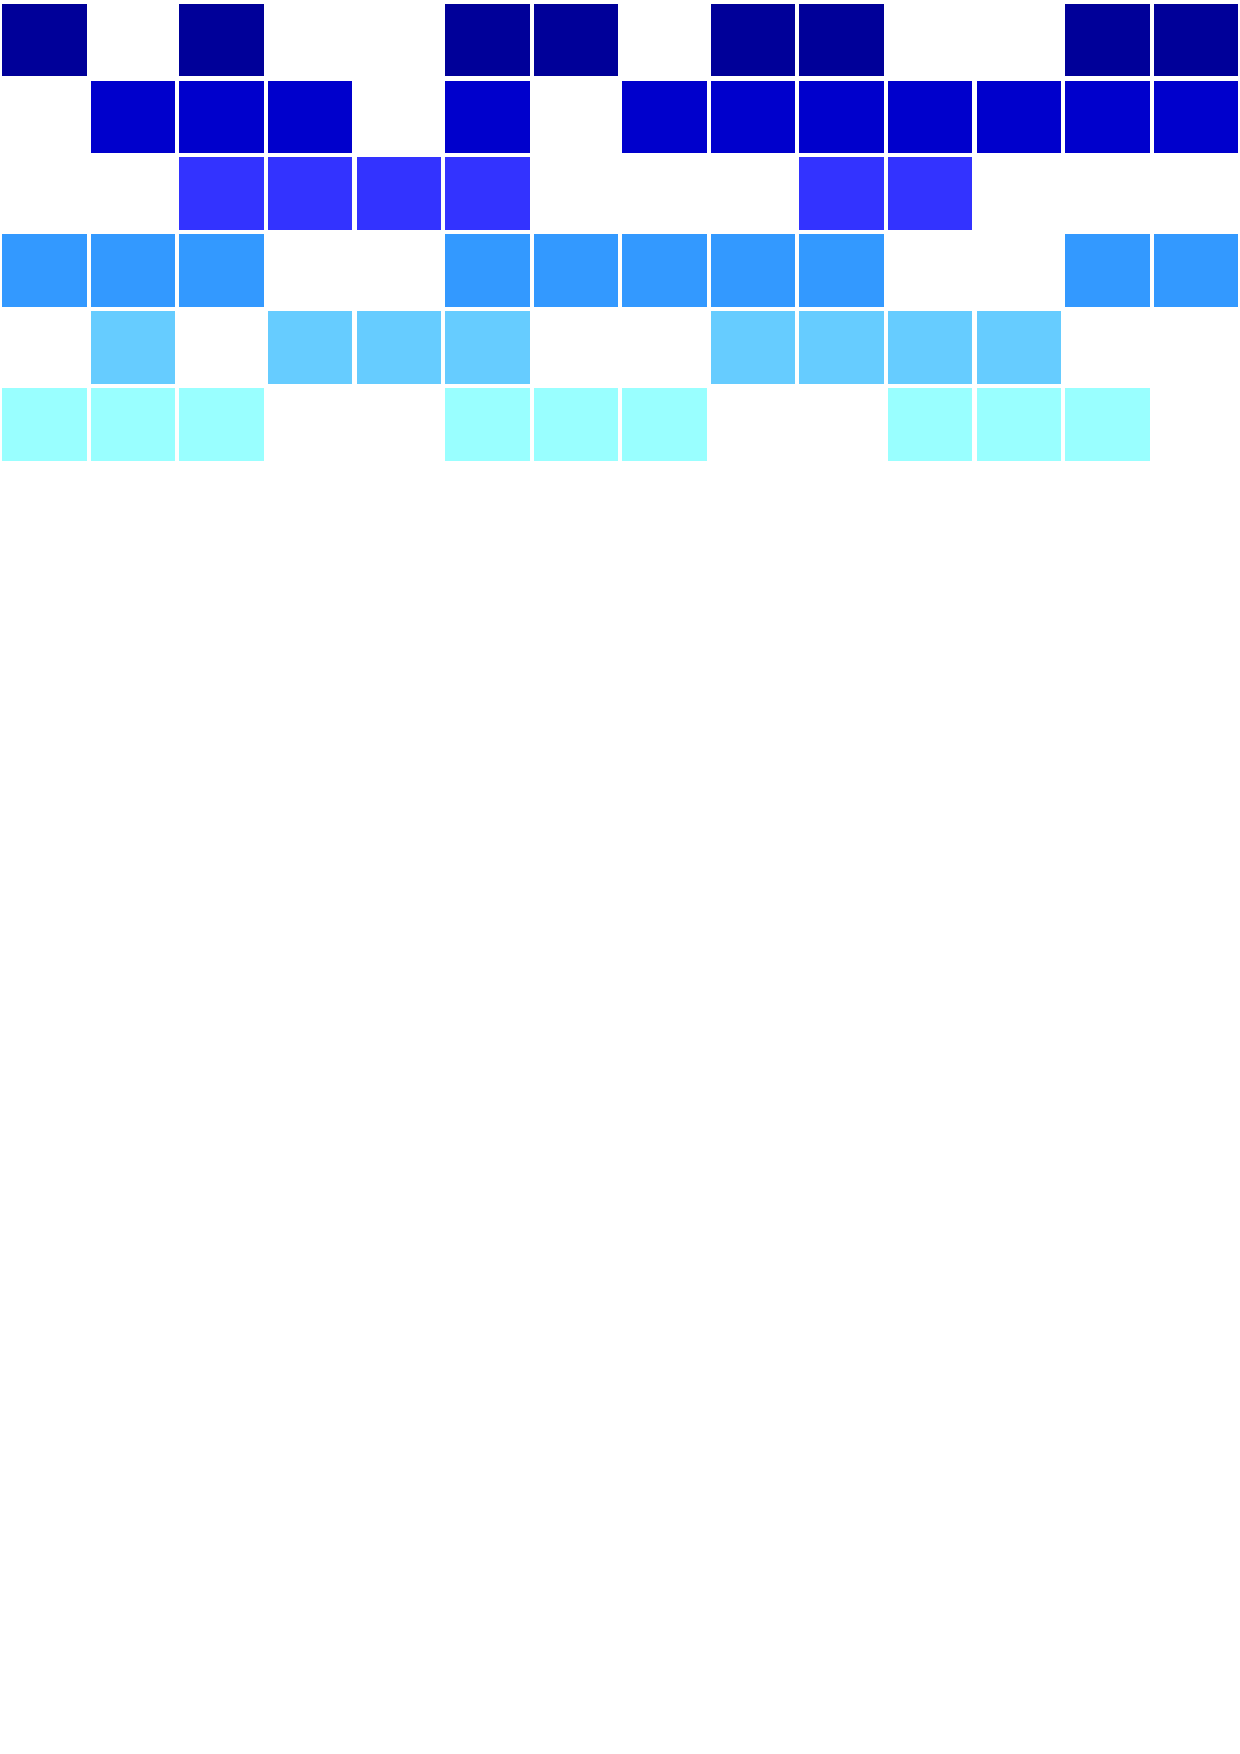
\includegraphics[width=\paperwidth]{background}}; % Background image
\draw[anchor=north] (midpoint) node [fill=ocre!30!white,fill opacity=0.6,text opacity=1,inner sep=1cm]{\Huge\centering\bfseries\sffamily\parbox[c][][t]{\paperwidth}{\centering Cálculo Diferencial e Integral\\[15pt] % Book title
{\Large Notas de Aula}\\[20pt] % Subtitle
{\huge Bruno de Araujo Coutinho}}}; % Author name
\end{tikzpicture}};
\end{tikzpicture}
\vfill
\endgroup


%----------------------------------------------------------------------------------------
%	TABLE OF CONTENTS
%----------------------------------------------------------------------------------------

%\usechapterimagefalse % If you don't want to include a chapter image, use this to toggle images off - it can be enabled later with \usechapterimagetrue

\chapterimage{chapter_head_1.pdf} % Table of contents heading image

\pagestyle{empty} % No headers

\tableofcontents % Print the table of contents itself

\cleardoublepage % Forces the first chapter to start on an odd page so it's on the right

\pagestyle{fancy} % Print headers again

%----------------------------------------------------------------------------------------
%	CHAPTER 1: Números Reais
%----------------------------------------------------------------------------------------
\chapterimage{chapter_head_2.pdf} % Chapter heading image
\chapter{Números Reais}

Os

%----------------------------------------------------------------------------------------
%	CHAPTER 2: Funções e Modelos
%----------------------------------------------------------------------------------------
\chapter{Funções e Modelos}

%----------------------------------------------------------------------------------------
%	CHAPTER 3: Limites e Continuidade
%----------------------------------------------------------------------------------------
\chapter{Limites e Continuidade}

Chama-se limite o comportamento de uma função $f(x)$ em torno de um valor $x$. Escrevemos
$$lim_{x \rightarrow a} f(x) = L$$
e dizemos "o limite de $f(x)$, quando $x$ tende a $a$ é igual a $L$" se pudermos tornar os valors de $f(x)$ arbitrariamente próximos de $L$ (tão próximos quanto quisermos), tornando $x$ suficientemente próximo de $a$ (por ambos os lados de $a$), mas não igual a $a$.

\begin{example}
Vamos investigar o comportamento de uma função $f$ definida por $f(x) = x^2 - x + 2$, para valores de $x$ próximos de 2.

\begin{tikzpicture}[scale=0.5]
\begin{axis}[
    axis lines = left,
    xlabel = $x$,
    ylabel = {$f(x)$},
]
%Below the red parabola is defined
\addplot [
    domain=0:3, 
    samples=100, 
    color=green,
]
{x^2 - x + 2};
\end{axis}
\end{tikzpicture}

\begin{table}
\begin{tabular}{|c|c||c|c|}
\hline
$x$ & $f(x)$ & $x$ & $f(x)$ \\
\hline 
1 & 2,000000 & 3 & 8,000000 \\
\hline
1,5 & 2,750000 & 2,5 & 5,750000 \\
\hline
1,9 & 3,710000 & 2,1 & 4,310000 \\
\hline
1,95 & 3,852500 & 2,05 & 4,152500 \\
\hline
1,99 & 3,970100 & 2,01 & 4,030099 \\
\hline
1,999 & 3,997001 & 2,001 & 4,003000 \\
\hline
\end{tabular}
\end{table}

\end{example}



%----------------------------------------------------------------------------------------
%	CHAPTER x: Integrais Múltiplas
%----------------------------------------------------------------------------------------
\chapter{Integrais Múltiplas}

\section{Integrais Duplas sobre Retângulos}

Se $f(x)$ é uma função de uma única variável real e é definida para $a \le x \le b$, subdividimos o intervalo $[a,b]$ em $n$ subintervalos $[x_{i-1},x_i]$ de comprimento igual a $\Delta x = (b-a)/n$ e escolhemos pontos arbitrários $x_i^{*}$ em cada um desses intervalos. Em seguida, formamos a soma de Riemann e tomamos o limite dessa soma quando $n \rightarrow \infty$ para oter a integral definida de $a$ até $b$ da função $f$

\begin{equation}
\lim_{n \rightarrow \infty} \sum_{i=1}^n f(x_i^*) \cdot \Delta x = \int_a^b f(x) dx
\end{equation}

\begin{figure}[!h]
 \centering
 \begin{tikzpicture}[xscale=1.2]
 %\draw [help lines] (0,0) grid (8,5);
 \draw [<->, thick] (0,5) -- (0,0) -- (8,0);
 \node [above] at (0,5) {$y$}; \node [right] at (8,0) {$x$}; 
 \draw[green, ultra thick, domain=0:8] plot (\x, {3+sin(deg(\x - 1))});
 \draw [blue] (1,0) rectangle (2,3.4794);
 \node [below] at (1,0) {$a$};
 \draw [blue] (2,0) rectangle (3,3.9975);
 \node [below] at (2,0) {$x_1$};
 \draw [blue] (3,0) rectangle (4,3.5985);
 \node [below] at (3,0) {$x_2$};
 \node [below] at (4,0) {$x_3$};
 \node at (4.5,1.5) {$\ldots$};
 \draw [blue] (5,0) rectangle (6,2.0225);
 \node [below] at (5,0) {$x_{i-1}$};
 \node [below] at (6,0) {$x_{i}$};
 \draw [blue] (6,0) rectangle (7,2.2945);
 \node [below] at (7,0) {$b$};
 \draw [|-|] (5,2.5) -- (6,2.5); \node [above] at (5.5,2.5) {$\Delta x$};
 \node [below=.3cm] at (5.5,0) {$x_i^*$};
 \draw [dotted] (5.5,-.3) -- (5.5,2.0225);
\end{tikzpicture}
 \caption{Somas de Riemman para funções de uma variável}
\end{figure}

De modo semelhante, considere uma função $f$ de duas variáveis definida em um retângulo fechado.

$$R = [a,b] \times [c,d] = \{ (x,y) \in \mathbb{R}^2 | a \le x \le b, c \le y \le d \} $$

O gráfico de $f$ é a superfície com equação $z = f(x,y)$. Seja $S$ o sólido contido acima de $R$ e abaixo da superfície $z$:

$$ S = \{ (x,y,z) \in  \mathbb{R}^3 | 0 \le z \le f(x,y), (x,y) \in R \} $$

\begin{figure}[!h]
 \centering
 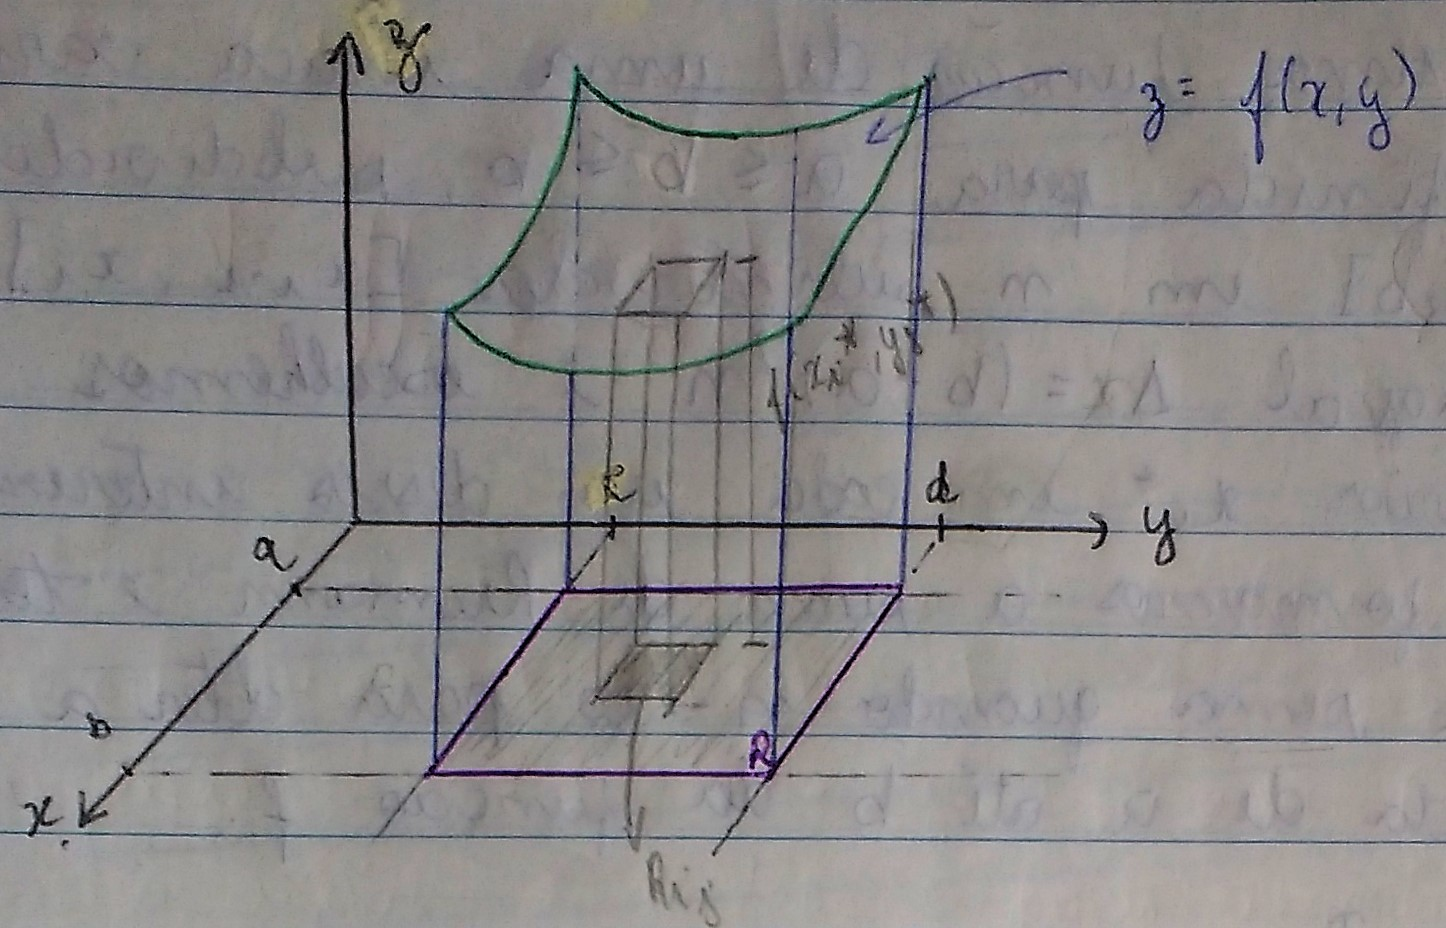
\includegraphics[width=10cm]{Pictures/graph2.jpg}
\end{figure}

Para determinar o volume de $S$, o primeiro passo é dividir o retângulo $R$ em sub-retângulos. Faremos isto dividindo o intervalo $[a,b]$ em $m$ subintervalos $[x_{i-1}, x_{i}]$ de mesmo comprimento $\delta x = (b-a)/m$ e o intervalo $[c,d]$ em $n$ subintervalos iguais $[y_{j-1}, y_{j}]$ de comprimento $\delta y = (d-c)/n$.

\begin{figure}[!h]
 \centering
 \begin{tikzpicture}
 %\draw [help lines] (0,0) grid (9,7);
 \draw [<->, thick] (0,7) -- (0,0) -- (9,0);
 %\node [above] at (0,5) {$y$}; \node [right] at (8,0) {$x$};
 \foreach \i in {1,...,8}
 {
  \draw [magenta] (\i,1) -- (\i,6);
  \draw [dotted] (\i,0) -- (\i,1);
 }
 \node [below] at (1,0) {$a$};
 \node [below] at (2,0) {$x_i$};
 \node [below] at (3,0) {$x_2$};
 \node [below=.1cm] at (4,0) {$\ldots$};
 \node [below] at (5,0) {$x_{i-1}$};
 \node [below=.1cm] at (7,0) {$\ldots$};
 \node [below] at (6,0) {$x_i$};
 \node [below] at (8,0) {$b$};
 \foreach \i in {1,...,6}
 {
  \draw [magenta] (1,\i) -- (8,\i);
  \draw [dotted] (1,\i) -- (0,\i);
 }
 \node [left] at (0,1) {$c$};
 \node [left] at (0,2) {$y_1$};
 \node [left] at (0,3) {$y_{j-1}$};
 \node [left] at (0,4) {$y_j$};
 \node [left] at (0,5) {$\vdots$};
 \node [left] at (0,6) {$d$};
 % labels y
 \path [fill=green!40] (5.05,3.05) rectangle (5.95,3.95);
 \draw [fill] (5.5,3.5) circle [radius=.1] node [above] {$(x_i^*, y_j^*)$};
 \draw [|-|] (5,0.5) -- (6,0.5); \node [below] at (5.5,0.5) {$\Delta x$};
 \draw [|-|] (0.5,3) -- (0.5,4); \node [right] at (0.5,3.5) {$\Delta y$};
\end{tikzpicture}
\end{figure}

Se escolhermos um ponto arbitrário em cada $R_{ij}$, $(x_i^*, y_j^*)$ definimos o volume da caixa de base $R_{ij}$ e altura $f(x_i^*, y_j^*)$ como:

$$ f(x_i^*, y_j^*) \cdot \Delta A $$

Se realizarmos este procedimento para os demais retângulos, vamos obter uma estimativa do volume:

$$ V \approx \sum_{i=1}^m \sum{j=1}^n f(x_i^*, y_j^*) \cdot \Delta A $$

A aproximação do volume acima melhora quando aumentamos os valores de $m$ e $n$, portanto:

$$ V = \lim_{m,n \rightarrow \infty} \sum_{i=1}^m \sum{j=1}^n f(x_i^*, y_j^*) \cdot \Delta A $$

Daí, podemos enunciar a definição de integral dupla sobre um retângulo $R_{ij}$.

\begin{definition}[Integral Dupla]
 A integral dupla de $f$ sobre o retângulo $R_{ij}$ é:
 \begin{equation}
  \iint _{R} f(x,y) dA = \lim_{m,n \rightarrow \infty} \sum_{i=1}^m \sum{j=1}^n f(x_i^*, y_j^*) \cdot \Delta A
 \end{equation}
 se este limite existir.
\end{definition}

O significado preciso da definição anterior é que para todo $\epsilon > 0$, existe um número $N$ talque

$$ \| \iint _{R} f(x,y) dA -  \lim_{m,n \rightarrow \infty} \sum_{i=1}^m \sum{j=1}^n f(x_i^*, y_j^*) \cdot \Delta A \| < \epsilon $$

para todos inteiros $m$ e $n$ maiores que $N$ e para qualquer escolha de $(x_i^*, y_j^*)$ em $R_{ij}$.



%----------------------------------------------------------------------------------------
%	CHAPTER 7: Análise da Potência CA
%----------------------------------------------------------------------------------------
%\chapter{Análise da Potência CA}

\section{Potência instantânea e potência média}

A \textbf{potência instantânea}, $p(t)$, em watts, é a taxa na qual um elemento absorve energia. É a potência a qualquer instante.

\begin{equation}
 p(t) = v(t) \cdot i(t)
\end{equation}

Considerando $v(t) = V_m cos(\omega t + \theta_v)$ e $i(t) = I_m cos(\omega t + \theta_i)$ e aplicando uma identidade trigonométrica \footnote{$cos(A)cos(B) = \frac{1}{2}cos(A-B) + \frac{1}{2}cos(A+B)$}, podemos expressar a potência como:

\begin{equation} \label{potinst}
 p(t) = \frac{1}{2}V_m I_m \cos(\theta_v - \theta_i) + \cos(2 \omega t + \theta_v + \theta_i)
\end{equation}

\begin{tikzpicture}
\begin{axis}[axis lines = left, xlabel = t (s), ylabel = V]
\addplot[domain=0:360,samples=100,color=red]{sin(x)};
\end{axis}
\end{tikzpicture}

A \textbf{potência média}, em watts, é a média da potência instantânea ao longo de um período.

\begin{equation}
 P = \frac{1}{2} \int_0^T p(t) dt
\end{equation}

Para a expressão na Equação \ref{potinst}, temos que:

\begin{equation}
 P = \frac{1}{2} V_m I_m cos(\theta_v - \theta_i)
\end{equation}

<demonstração>

Note que $p(t)$ cvaria com o tempo, ao passo que $P$ não.

As formas fasoriais de $v(t)$ e $i(t)$  são, respectivamente, $\mathbf{V} = V_m \angle \theta_v$ e $\mathbf{I} = I_m \angle \theta_i$. Para usar fasores, percebemos que:

\begin{align}
 \frac{1}{2} \mathbf{V}\mathbf{I^*} &= \frac{1}{2} = V_m I_m \angle \theta_v - \theta_i \\
 &= \frac{1}{2} V_m I_m [\cos(\theta_v - \theta_i) + j \sin(\theta_v - \theta_i)]
\end{align}

Reconhecemos a parte real dessa expressão como a potência média, P.

Em um circuito resistivo, $\theta_v = \theta_i$, então, $\cos(\theta_v - \theta_i) = 1$, nos dando

\begin{equation}
 P = \frac{1}{2} V_m I_m = \frac{1}{2} {I_m}^2 R
\end{equation}

Quando $\theta_v - \theta_i = +- 90^{\circ}$, temos que $\cos(\theta_v - \theta_i) = 0$. Então, em um circuito putamente reativo, a potência média é zero.

<3 exemplos>

\section{Transferência de Potência média Máxima}

Considere o equivalente de Thévenin de um circuito:

<figura>

Na morma retangular, as impedâncias são:

\begin{align}
 Z_{Th} &= R_{Th} + j X_{Th} \\
 Z_L &= R_L + j X_L
\end{align}

A corrente através da carga será:

\begin{equation}
 \mathbf{I} = \frac{\mathbf{V}_{Th}}{Z_{Th} + Z_L} = \frac{\mathbf{V}_{Th}}{(R_{Th} + R_L) + j (X_{Th} + X_L)}
\end{equation}

A potência média na carga então será

\begin{equation} \label{potencia}
 P = \frac{1}{2} |\mathbf{I}|^2 \cdot R_L = \frac{|\mathbf{V}_{Th}| R_L / 2}{(R_{Th} + R_L)^2 + (X_{Th} + X_L)^2}
\end{equation}

Tomando $\partial P / \partial R_L$ e $\partial P / \partial X_L$ e igualando ambas expressões a zero, vamos ter:

%\begin{align}
% X_L &= - X_{Th} \label \\
% R_L &= \sqrt{{R_{Th}}^2 + (X_{Th} + X_L)^2}
%\end{align}

Combinando as Equações, conclui-se que para haver a máxima transferência,

\begin{equation}
 Z_L = {Z_{Th}}^{*}
\end{equation}

Fazendo $Z_L = {Z_{Th}}^{*}$ na Equação \eqref{potencia}, vamos obter a potência média máxima na carga:

\begin{equation}
 P_{\text{máx}} = \frac{|\mathbf{V}_{Th}|^2}{8 R_{Th}} 
\end{equation}

<exemplos>

\section{Valor Eficaz ou RMS}

\textbf{Valor eficaz} de uma corrente periódica é a corrente


% 4 Derivadas
% 5 Aplicações de Derivadas
% 6 Integrais
% 7 Aplicações de Integrais
% 8 Tecnicas de Integração
% 9 Séries
% 10 Derivadas Parciais
% 11 Integrais Múltiplas
%----------------------------------------------------------------------------------------
%	BIBLIOGRAPHY
%----------------------------------------------------------------------------------------

\chapter*{Bibliography}
\addcontentsline{toc}{chapter}{\textcolor{ocre}{Bibliography}}
\section*{Books}
\addcontentsline{toc}{section}{Books}
\printbibliography[heading=bibempty,type=book]
\section*{Articles}
\addcontentsline{toc}{section}{Articles}
\printbibliography[heading=bibempty,type=article]

%----------------------------------------------------------------------------------------
%	INDEX
%----------------------------------------------------------------------------------------

\cleardoublepage
\phantomsection
\setlength{\columnsep}{0.75cm}
\addcontentsline{toc}{chapter}{\textcolor{ocre}{Index}}
\printindex

%----------------------------------------------------------------------------------------

\end{document}
